%------------------------------------------------------------------------------
\chapter{Useful information}
\label{sec:app}
%------------------------------------------------------------------------------

\section{MC Dijet Slices}
Truth $p_\mathrm{T}$ of jet given by anti-$k_\mathrm{T}$ jet algorithm with distance parameter $R=0.6$:
\begin{itemize}
\item[JZ0W] 0 - 20 GeV
\item[JZ1W] 20 - 60 GeV
\item[JZ2W] 60 - 160 GeV
\item[JZ3W] 160 - 400 GeV
\item[JZ4W] 400 - 800 GeV
\item[JZ5W] 800 - 1300 GeV
\item[JZ6W] 1300 - 1800 GeV
\item[JZ7W] 1800 - 2500 GeV
\item[JZ8W] 2500 - 3200 GeV
\end{itemize}

\url{https://svnweb.cern.ch/cern/wsvn/atlasoff/Generators/MC15JobOptions/trunk/share/DSID361xxx/MC15.361021.Pythia8EvtGen_A14NNPDF23LO_jetjet_JZ1W.py}


\url{https://svnweb.cern.ch/cern/wsvn/atlasoff/Generators/MC15JobOptions/trunk/common/Filters/JetFilterAkt6.py}


\url{https://svnweb.cern.ch/cern/wsvn/atlasoff/Generators/MC15JobOptions/trunk/common/Filters/JetFilter_JZX_Fragment.py}

\subsection{Preproduction Taus}

\begin{lstlisting}[basicstyle=\small\ttfamily, breaklines=true]
mc16_13TeV.425200.Pythia8EvtGen_A14NNPDF23LO_Gammatautau_MassWeight.merge.AOD.e5468_s2997_r9064_r8996
\end{lstlisting}

\subsection{MC16A Taus}

\begin{lstlisting}[basicstyle=\small\ttfamily, breaklines=true]
mc16_13TeV.425200.Pythia8EvtGen_A14NNPDF23LO_Gammatautau_MassWeight.merge.AOD.e5468_s3126_r9364_r9315
\end{lstlisting}

\subsection{Preproduction Dijets}

\begin{lstlisting}[basicstyle=\small\ttfamily, breaklines=true]
mc16_13TeV.361021.Pythia8EvtGen_A14NNPDF23LO_jetjet_JZ1W.merge.AOD.e3569_s2997_r9064_r8996
mc16_13TeV.361022.Pythia8EvtGen_A14NNPDF23LO_jetjet_JZ2W.merge.AOD.e3668_s2997_r9064_r9078
mc16_13TeV.361023.Pythia8EvtGen_A14NNPDF23LO_jetjet_JZ3W.merge.AOD.e3668_s2997_r9064_r8996
mc16_13TeV.361024.Pythia8EvtGen_A14NNPDF23LO_jetjet_JZ4W.merge.AOD.e3668_s2997_r9064_r9078
mc16_13TeV.361025.Pythia8EvtGen_A14NNPDF23LO_jetjet_JZ5W.merge.AOD.e3668_s2997_r9064_r8996
mc16_13TeV.361026.Pythia8EvtGen_A14NNPDF23LO_jetjet_JZ6W.merge.AOD.e3569_s2997_r9064_r9078
\end{lstlisting}


\clearpage
\section{Tau-ID Variables}

\subsection{1-prong}
\begin{figure}[!ht]
  \begin{subfigure}{0.5\textwidth}
    \centering
    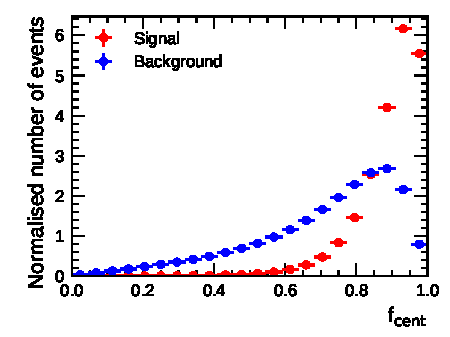
\includegraphics{./figures/baseline_bdt_vars/1p/centFrac.pdf}
  \end{subfigure}%
  \begin{subfigure}{0.5\textwidth}
    \centering
    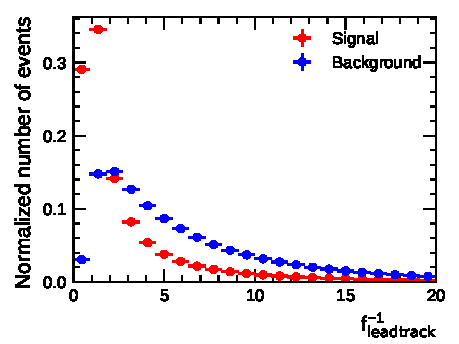
\includegraphics{./figures/baseline_bdt_vars/1p/etOverPtLeadTrk.pdf}
  \end{subfigure}
  \begin{subfigure}{0.5\textwidth}
    \centering
    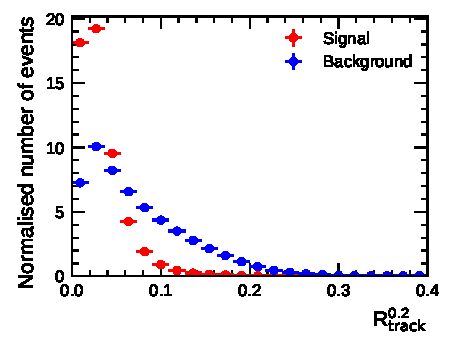
\includegraphics{./figures/baseline_bdt_vars/1p/innerTrkAvgDist.pdf}
  \end{subfigure}%
  \begin{subfigure}{0.5\textwidth}
    \centering
    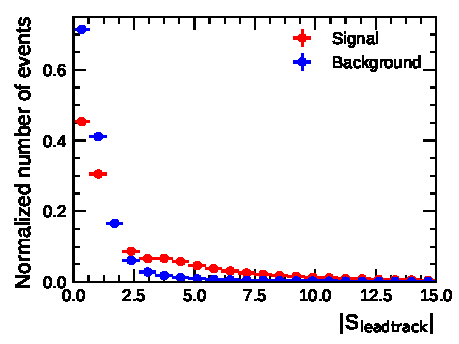
\includegraphics{./figures/baseline_bdt_vars/1p/absipSigLeadTrk.pdf}
  \end{subfigure}
  \begin{subfigure}{0.5\textwidth}
    \centering
    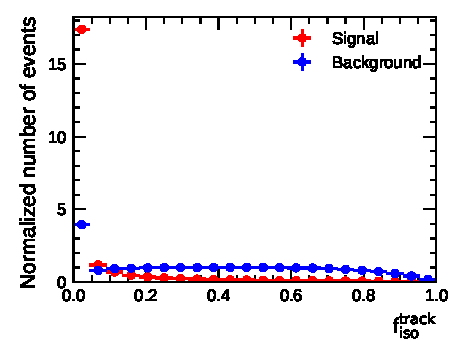
\includegraphics{./figures/baseline_bdt_vars/1p/SumPtTrkFrac.pdf}
  \end{subfigure}%
  \begin{subfigure}{0.5\textwidth}
    \centering
    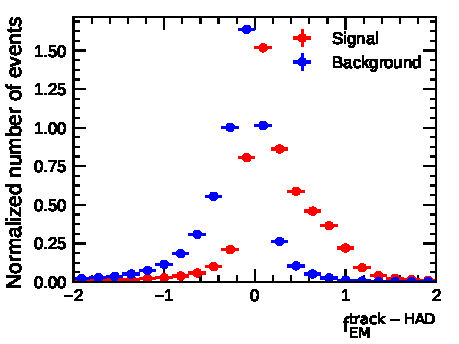
\includegraphics{./figures/baseline_bdt_vars/1p/ChPiEMEOverCaloEME.pdf}
  \end{subfigure}
  \caption{Variables used in Tau-ID BDT}
  \label{fig:bdt_vars_1p_overlays}
\end{figure}

\begin{figure}[!ht]\ContinuedFloat
  \begin{subfigure}{0.5\textwidth}
    \centering
    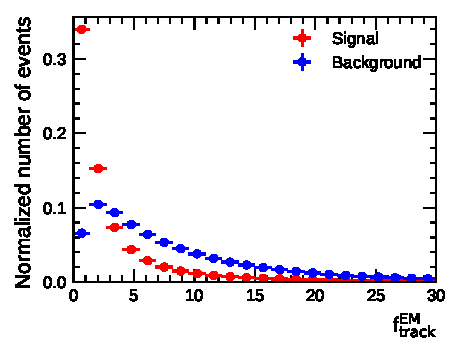
\includegraphics{./figures/baseline_bdt_vars/1p/EMPOverTrkSysP.pdf}
  \end{subfigure}%
  \begin{subfigure}{0.5\textwidth}
    \centering
    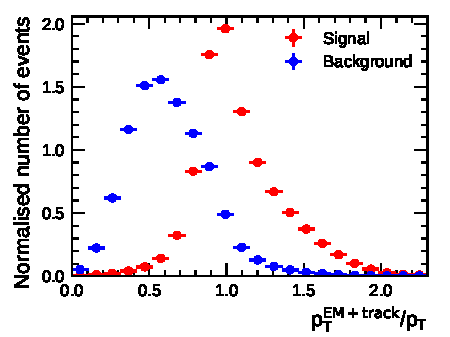
\includegraphics{./figures/baseline_bdt_vars/1p/ptRatioEflowApprox.pdf}
  \end{subfigure}
  \begin{subfigure}{0.5\textwidth}
    \centering
    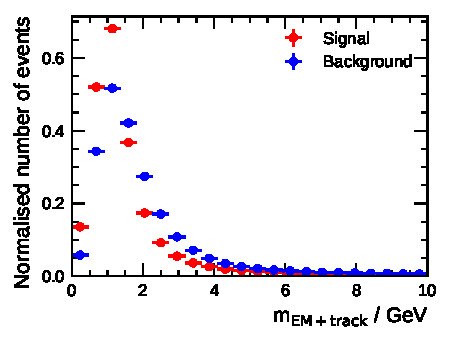
\includegraphics{./figures/baseline_bdt_vars/1p/mEflowApprox.pdf}
  \end{subfigure}
  \caption[]{Variables used in Tau-ID BDT}
\end{figure}

\clearpage
\subsection{3-prong}

\begin{figure}[!ht]
  \begin{subfigure}{0.5\textwidth}
    \centering
    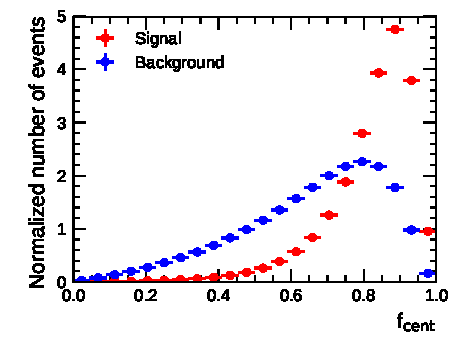
\includegraphics{./figures/baseline_bdt_vars/3p/centFrac.pdf}
  \end{subfigure}%
  \begin{subfigure}{0.5\textwidth}
    \centering
    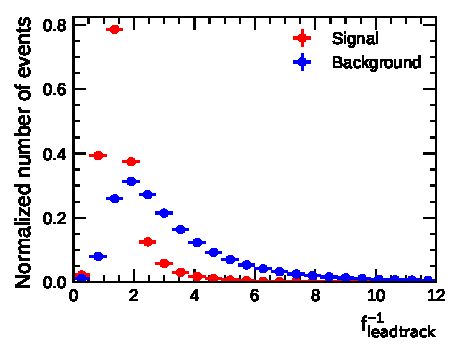
\includegraphics{./figures/baseline_bdt_vars/3p/etOverPtLeadTrk.pdf}
  \end{subfigure}
  \begin{subfigure}{0.5\textwidth}
    \centering
    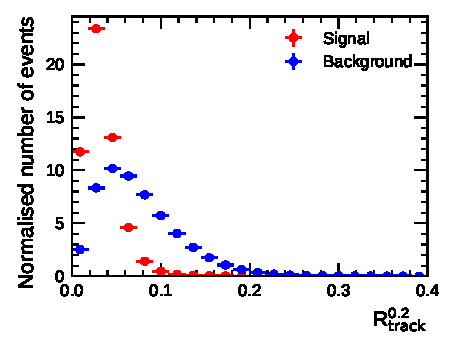
\includegraphics{./figures/baseline_bdt_vars/3p/innerTrkAvgDist.pdf}
  \end{subfigure}%
  \begin{subfigure}{0.5\textwidth}
    \centering
    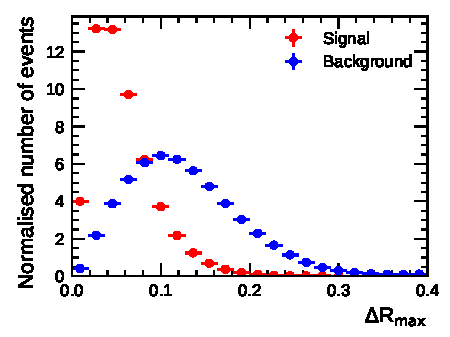
\includegraphics{./figures/baseline_bdt_vars/3p/dRmax.pdf}
  \end{subfigure}
  \begin{subfigure}{0.5\textwidth}
    \centering
    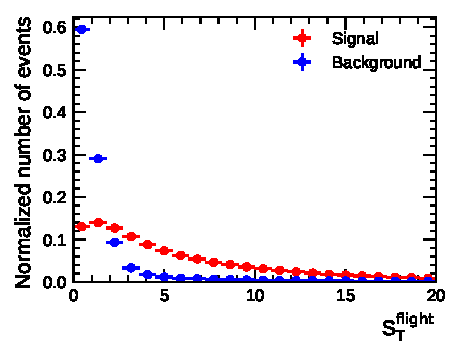
\includegraphics{./figures/baseline_bdt_vars/3p/trFlightPathSig.pdf}
  \end{subfigure}%
  \begin{subfigure}{0.5\textwidth}
    \centering
    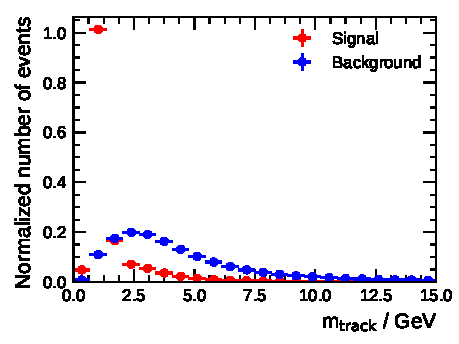
\includegraphics{./figures/baseline_bdt_vars/3p/massTrkSys.pdf}
  \end{subfigure}
  \caption{Variables used in Tau-ID BDT}
  \label{fig:bdt_vars_3p_overlays}
\end{figure}

\begin{figure}[!ht]\ContinuedFloat
  \begin{subfigure}{0.5\textwidth}
    \centering
    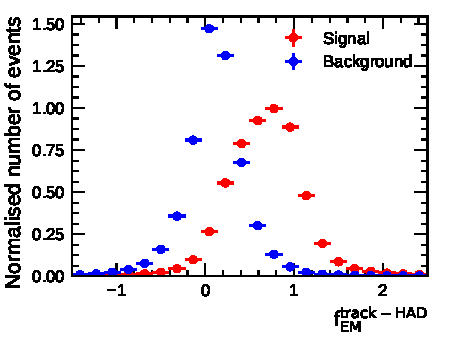
\includegraphics{./figures/baseline_bdt_vars/3p/ChPiEMEOverCaloEME.pdf}
  \end{subfigure}%
  \begin{subfigure}{0.5\textwidth}
    \centering
    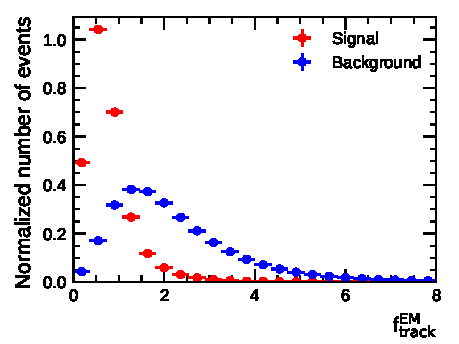
\includegraphics{./figures/baseline_bdt_vars/3p/EMPOverTrkSysP.pdf}
  \end{subfigure}
  \begin{subfigure}{0.5\textwidth}
    \centering
    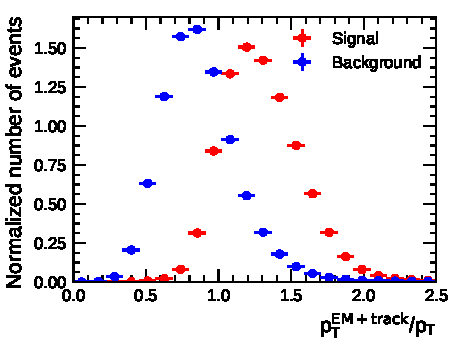
\includegraphics{./figures/baseline_bdt_vars/3p/ptRatioEflowApprox.pdf}
  \end{subfigure}%
  \begin{subfigure}{0.5\textwidth}
    \centering
    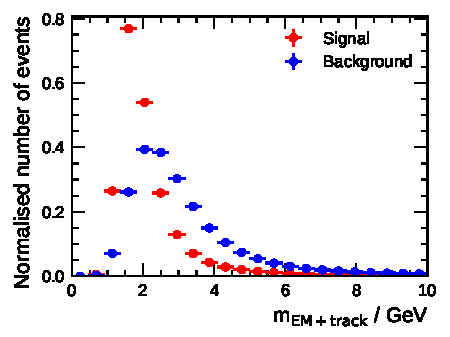
\includegraphics{./figures/baseline_bdt_vars/3p/mEflowApprox.pdf}
  \end{subfigure}
  \caption[]{Variables used in Tau-ID BDT}
\end{figure}


%%% Local Variables:
%%% mode: latex
%%% TeX-master: "mythesis"
%%% End:
